\documentclass[preprint,11pt,a4paper]{elsarticle}
\usepackage[T1]{fontenc}
\usepackage[utf8]{inputenc}
\usepackage[margin=25mm]{geometry}
\usepackage{amsmath,amssymb,booktabs,graphicx}
\usepackage[colorlinks=true,urlcolor=blue,citecolor=blue,linkcolor=black]{hyperref}
\usepackage{url}
\makeatletter
\def\ps@pprintTitle{\let\@oddhead\@empty\let\@evenhead\@empty
  \def\@oddfoot{\footnotesize Roland Cédric TAYO --- Teaching manuscript\hfill\thepage}
  \let\@evenfoot\@oddfoot}
\makeatother
\setlength{\parskip}{3pt}
\setlength{\emergencystretch}{2em}
\begin{document}

\begin{frontmatter}
\title{From a small forecasting network to a measurable embedded experiment}
\author{Roland Cédric TAYO}
\address{AI for Embedded Systems, 2026--2027}
\begin{abstract}
Deploying a predictor on a small board requires more than reporting its prediction error. The implementation must also be correct, fit in memory and execute within a measured time budget. This teaching manuscript illustrates how to report a hand-written forecasting network inspired by TSMixer and how to design an experiment on its dense projections. It provides an architecture diagram, an independently generated signal illustration and analytical parameter counts. It deliberately reports no network training results and no measurements from a microcontroller. Its purpose is to demonstrate the structure of an article and the distinction between calculated quantities, observed data and untested hypotheses. A final student report must replace these illustrations with traceable training and hardware experiments. Negative findings remain useful when the protocol is correct and the scope of the conclusion is explicit.
\end{abstract}
\begin{keyword}
Embedded inference \sep time-series forecasting \sep dense projection \sep reproducibility
\end{keyword}
\end{frontmatter}

\section{Introduction}
A device can use recent observations to estimate the next value without sending its data to a server. Local inference can reduce dependence on a network connection, but it consumes memory and computation on the device. A small numerical model is therefore useful only when its accuracy and execution cost satisfy the actual application requirements.

This manuscript is a \textbf{format example}, not a completed project or a publication claim. Its research question is: \emph{under fixed weights and inputs, can a different organisation of a dense projection reduce execution cost on a chosen board?} One possible hypothesis is that computing several output values together reuses input loads. This may help for some shapes and hurt for others because of register pressure or additional code. No improvement is assumed in advance.

\section{Background and scope}
TSMixer combines mixing across time and across variables using multilayer perceptrons \cite{chen2023tsmixer}. The TD uses a deliberately reduced residual network rather than a reproduction of the published model. Shared parameters and manual differentiation expose the main numerical mechanisms without requiring a framework. Gradient checks help detect implementation mistakes before training \cite{cs231n}.

CMSIS-NN provides optimised kernels for Cortex-M processors \cite{armcmsis}. It can serve as a separately labelled comparator when the target and operation match. It does not establish a portable performance target for every floating-point implementation. Quantisation is another research direction \cite{jacob2018quantization}, but it changes numerical behaviour and is outside the mandatory loop-organisation study.

\section{Method}
\subsection{Predictor and dimensions}
The input $X\in\mathbb{R}^{16\times3}$ contains sixteen successive samples of three variables. Here $\mathbb{R}$ denotes real-valued entries. The first mixing stage uses shared temporal weights; the second uses shared feature weights. Both add a learned correction to their input. A linear head produces one next-step estimate (Figure~\ref{fig:architecture}).
\begin{figure}[htbp]
\centering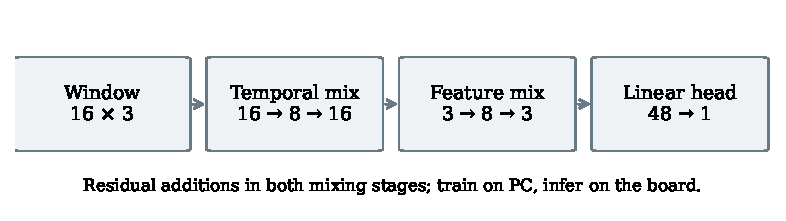
\includegraphics[width=\linewidth]{figures/architecture.pdf}
\caption{Pedagogical network. Arrows indicate data flow, not measured runtime. This is a reduced adaptation of TSMixer, not the full published architecture.}
\label{fig:architecture}
\end{figure}

The temporal stage has $8\times16+8+16\times8+16=280$ parameters. The feature stage has $8\times3+8+3\times8+3=59$. The output head has $48+1=49$. Therefore,
\begin{equation}
n_{\mathrm{param}}=280+59+49=388,\qquad
M_{\mathrm{weights}}=4n_{\mathrm{param}}=1552\ \mathrm{bytes}.
\label{eq:memory}
\end{equation}
Here $n_{\mathrm{param}}$ is the total number of trainable scalar parameters; $M_{\mathrm{weights}}$ is their payload when each occupies four bytes (float32). It is not a measurement of total SRAM or Flash. Activations, stack, code, runtime and alignment must be assessed separately.

\subsection{Dense operation and candidate change}
For an input vector $x$ of length $n_{\mathrm{in}}$ and an output vector $z$ of length $n_{\mathrm{out}}$, the dense projection is
\begin{equation}
z_j=b_j+\sum_{k=1}^{n_{\mathrm{in}}}W_{j,k}x_k,
\quad j=1,\ldots,n_{\mathrm{out}}.
\label{eq:dense}
\end{equation}
$W$ is a matrix with $n_{\mathrm{out}}$ rows and $n_{\mathrm{in}}$ columns; $b$ is the bias vector. Indices $j$ and $k$ identify an output and an input. The summation sign means adding every product over the stated range. A candidate implementation changes loop order or groups outputs while keeping the same mathematical function. Changing arithmetic order can change floating-point rounding, so correctness must be checked before timing.

\subsection{Signal illustration, distinct from TD data}
Figure~\ref{fig:signal} uses 100 samples of a sine wave plus Gaussian noise generated with NumPy's default generator seeded with 2026. This trace is \textbf{not} the TD simulator, training set, validation set or reserved test set. It only demonstrates plotting and a simple persistence predictor. The CSV and plotting source are included with the article.
\begin{figure}[htbp]
\centering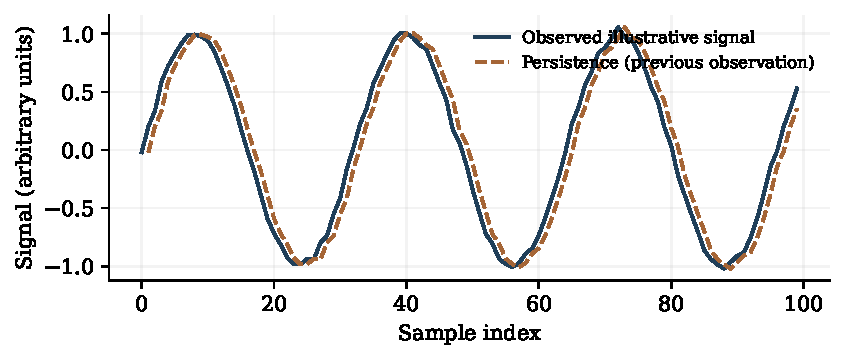
\includegraphics[width=\linewidth]{figures/illustrative_signal.pdf}
\caption{A separate illustrative trace and persistence predictions. The prediction for sample $i$ is the observation at sample $i-1$. These are not predictions from a trained network and contain no hardware measurements.}
\label{fig:signal}
\end{figure}

For $N$ evaluated predictions, mean squared error (MSE) and mean absolute error (MAE) are
\begin{equation}
\mathrm{MSE}=\frac{1}{N}\sum_{i=1}^{N}(\hat y_i-y_i)^2,
\qquad
\mathrm{MAE}=\frac{1}{N}\sum_{i=1}^{N}|\hat y_i-y_i|.
\end{equation}
$y_i$ denotes the observed target; $\hat y_i$ is its prediction, marked by a hat. Absolute-value bars remove the sign. The first sample has no preceding observation, giving $N=99$ evaluated predictions. MSE has squared signal units; MAE has signal units. No classification accuracy is defined for this regression task.

\section{Proposed hardware protocol}
Before optimisation, the final report must identify the exact board, processor, frequency, memory, compiler and flags. Inputs, weights and preprocessing statistics are frozen and hashed. PC and board outputs are compared using the same windows. A tolerance and the numerical scale of comparison must be stated.

Time only the intended operation. Keep serial output outside that interval, retain a checksum to prevent dead-code elimination and repeat short operations until the timer resolution is adequate. Run at least three independent campaigns, alternate reference and candidate order, and retain raw repetitions. Report the median and a named dispersion statistic. Separate preparation costs, isolated projection costs and full-network inference costs.

If $T_{\mathrm{ref}}>0$ and $T_{\mathrm{var}}>0$ are reference and variant costs in the same unit, define
\begin{equation}
S=\frac{T_{\mathrm{ref}}}{T_{\mathrm{var}}},\qquad
G=100\frac{T_{\mathrm{ref}}-T_{\mathrm{var}}}{T_{\mathrm{ref}}}\ \%.
\end{equation}
$S$ is speedup and $G$ is time saved as a percentage. A ratio computed from PC timings cannot substitute for a measurement on the target board. No energy value should be reported without a suitable measurement method.

\section{Illustrative results and missing evidence}
Table~\ref{tab:results} separates analytical quantities and calculations on the illustrative trace from experiments that have not been performed. It intentionally leaves hardware and network-training results unresolved. The persistence metrics can be recomputed from the supplied CSV without any training code.
\begin{table}[htbp]
\centering\small
\begin{tabular}{p{.42\linewidth}p{.20\linewidth}p{.25\linewidth}}
\toprule Quantity & Value & Evidence type \\
\midrule
Trainable parameters & 388 & Analytical count \\
float32 parameter payload & 1552 bytes & Analytical count \\
Illustrative persistence MSE & 0.020976 & CSV calculation \\
Illustrative persistence MAE & 0.128263 & CSV calculation \\
Trained-network test error & Not measured & Requires training \\
Board inference cycles & Not measured & Requires hardware \\
Peak SRAM and energy & Not measured & Requires method \\
\bottomrule
\end{tabular}
\caption{Demonstration results. Signal units are arbitrary; MSE uses their square. No values in this table claim an optimisation gain or a microcontroller measurement.}
\label{tab:results}
\end{table}

\section{Discussion and next experiment}
The parameter count establishes only that the learned payload is small. It does not prove that the program fits in a particular board, respects a deadline or saves energy. Likewise, a persistence result on a simple sine wave does not establish the usefulness of a neural network on an industrial process.

A useful next experiment would compare a scalar reference against a two-output grouped projection for fixed $16\!\rightarrow\!8$, $32\!\rightarrow\!16$ and $64\!\rightarrow\!32$ shapes. These denote input and output lengths, respectively. First verify numerical equivalence, then collect alternating hardware timing campaigns. Integrate the change into the actual network only for its real shapes. The hypothesis would be weakened if the apparent gain disappeared across campaigns or was cancelled by preparation cost. A small isolated gain may also have a negligible end-to-end effect.

\section{Conclusion}
An embedded-learning experiment should connect model correctness, prediction quality and resource measurements. This example demonstrates how to state the question and distinguish known quantities from missing evidence. The student's contribution will be the tested implementation, the target-specific investigation and a justified next question, rather than a guaranteed positive gain.

\section*{Reproducibility and contributions}
The accompanying archive contains this source, a student template, references, vector figures, an illustrative CSV and the plotting script. It contains no implemented TD model, training loop or hardware firmware. The plotting script recomputes the illustrative metrics. A final submission must additionally name its GitHub repository, release tag, experiment manifests and commands. All authors should declare their contributions, reused code and substantial assistant usage. This document is a prepared teaching example and must not be presented as original student experimental work.

\bibliographystyle{elsarticle-num}
\bibliography{references}
\end{document}
